\documentclass[tikz,border=2pt]{standalone}
\usepackage{tikz}
\usetikzlibrary{positioning}
\begin{document}
	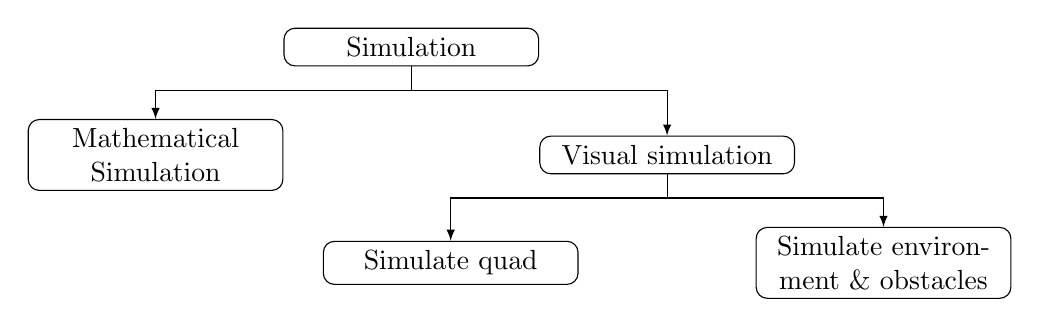
\begin{tikzpicture}[
	main/.style={rectangle, rounded corners, text centered, text width=3cm, draw=black},
	aux/.style={}
	]	
		
		\node (sim) [main] {Simulation};
			\node (aux2) [aux, below=of sim] {};
			\node (mathsim) [main, left=1.5cm of aux2] {Mathematical Simulation};
			\node (visualsim) [main, right=1.5cm of aux2] {Visual simulation};
				\node (aux6) [aux, below=of visualsim] {};
				\node (simulatequad) [main, left=of aux6] {Simulate quad};
				\node (simulateenvironm) [main, right=of aux6] {Simulate environment \& obstacles};
	
	
	\draw [-latex] (sim.south)--++(0,-.3)-| (mathsim.north);
	\draw [-latex] (sim.south)--++(0,-.3)-| (visualsim.north);
	\draw [-latex] (visualsim.south)--++(0,-.3)-| (simulatequad.north);	
	\draw [-latex] (visualsim.south)--++(0,-.3)-| (simulateenvironm.north);	
	
	\end{tikzpicture}
\end{document}